\documentclass[a4paper]{scrreprt}

% Anpassung des Seitenlayouts ----------------------------------------------
% 	siehe style.tex
% 

%
% Deutsche Sprache
%
\usepackage[german]{babel}

%
% ermöglicht ä, ö, ü und ß einzugeben
%
\usepackage[utf8]{inputenc}
%\usepackage[T1]{fontenc}
% Modernere Schrift
%\usepackage{lmodern}
%
\usepackage{graphicx}

%
% Formatierung von Listings.
%
\usepackage{listings}
\lstset{basicstyle=\small}


%
% bunt
%
\usepackage{color}

%\usepackage{multicol}


%\usepackage{multirow}

%
% bunte Tabellen.
%
\usepackage{colortbl}

%
% Mathematische Symbole
%
\usepackage{amsmath,amsthm,amssymb}


%\usepackage{floatflt}

%
% Fancy Kopf- und Fußzeile
%
%\usepackage{fancyhdr}
\usepackage{scrpage2}

%
% for testing purposes
%
\usepackage{blindtext}

%
% Benutzung von Links in PDF-Dokumenten.
%
\usepackage{hyperref}
\hypersetup{
colorlinks=false,
linkbordercolor={1 0 1},
pdfborder={0 0 0}
}

% n Bildchen nebeneinander
\usepackage{subfigure}

% Bildchen auf komplizierte Art selber malen
\usepackage{pstricks}
\usepackage{pst-node}


% Für die Ränder der Seite
\usepackage{geometry}

% vernünftige Zitate
\usepackage[square,comma,numbers]{natbib}

\usepackage{algorithmic}
\usepackage{algorithm}

\usepackage{setspace}

\usepackage{helvet}

\usepackage{lineno}


\begin{document}
\thispagestyle{empty}
\begin{center}
\vspace*{\fill}{\includegraphics[scale=0.7]{images/iais_85mm_p334.eps} \hfill 
\includegraphics[scale=0.07]{images/uni-bonn_logo}}
\vfill {Diplomarbeit an der Rheinischen Friedrich-Wilhelms-Universität Bonn \\ \vspace{16pt}
\huge \textbf{Die Untersuchung von thematischen Zentralitätsverläufen in Textsequenzen} \\ \vspace{16pt}\Large Centime \\\vspace{12pt}\begin{normalsize}vorgelegt von Florian Schulz\end{normalsize}}
\end{center}

\vfill {$\;$%\makebox[\textwidth][c]{% exchange [l] with [r] or [c] to extend it into the left border or both, respectively
%\includegraphics[width=1.46\textwidth]{images/run}
 %}
}
\vfill {$\;$}
\end{document}